\chapter{Behavioural graph models}\label{sec:users-behaviors}

If we want to infer some information about a graph that is particularly big, such as the ones behind the web or social networks like Facebook, we usually can't perform most tasks directly on the actual graph: in the majority of cases, such tasks would take too much time. For this reason, graph models are devised in order to represent the actual ones closely enough, and then are used in their stead to perform efficient analysis.

Some properties are of recurrent interest when dealing with a network:
\begin{itemize}
    \item the overall number of nodes,
    \item the average degree,
    \item the number of nodes with a certain degree,
    \item the size of the ``communities'',
    \item the degree distribution.
\end{itemize}

\section{Erd\H{o}s–Rényi model}\label{sec:gnp}
    
This is a model for generating random graphs, that has many applications due to its simplicity, but doesn't fit real world networks: the nodes in such a generated graph have more or less the same degree, based on a fixed probability; in real networks degrees usually follow a Gaussian distribution.

Denote by $\ergen(n, p)$ a random process that produces a graph with $n$ nodes, in which each edge appears with probability $p$. This process can be described by the following algorithm:

\begin{lstlisting}[caption = {The $\ergen(n,p)$ algorithm}, label = {lst:gnp}]
algorithm $\ergen(n,p)$:
    $V \gets [n]$
    $E \gets \emptyset$
    $\forall \{i, j\} \in \binom{V}{2}$:
        $b \pickUAR \coin(p)$
        if $b = 1$:
            $E \gets E \cup \{\{i,j\}\}$
    return $G := (V, E)$
\end{lstlisting}

Note that the probability $p$ is the same for all edges; the interest lies in studying how it influences the graphs generated by the process.
    

\subsubsection{Degree distribution}\label{sec:gnp-degree}

We begin our study of a given graph $G = (V, E)$ obtained by $\ergen(n, p)$ by looking at its degree distribution. Let $X = \deg(i) = \sum_{j \neq i} X_j$, where $i$ and $j$ are vertices, and the $X_j$ are mutually independent RVs defined as:
\[
    X_j =
    % TODO More ampersands are not accepted by 'cases', requires 'multi-column' env
    \begin{cases}
        1 & \text{if } \exists i : \{i, j\} \in E(G) \text{\qquad (with probability } p)                    \\
        0 & \text{otherwise}                         \text{\qquad \qquad \qquad (with probability } 1 - p)  \\
    \end{cases}
\]
Observe that $X$ is the same regardless of the chosen vertex $i$, since all probabilities do not change by changing $i$. Also, note that from the perspective of $i$, there are $\abs{V} - 1$ possible edges coming out of it, and are all governed by the same distribution; therefore:
\[
    \expect(\deg(i)) = \sum_{j \neq i} \Pr[\{i, j\} \in E(G)] = \sum_{j \neq i} p = (n - 1) p
\]

\todo{
    It can be valuable to get a better visual in how the degree distributes, or better, to discover that it is actually \emph{concentrated} around the average. Thanks to the mutual independence of the $x_j$, we can apply the Chernoff Bound [\ref{chernoff2}] to prove such claim:
    \[
        \Pr\left[X = \frac{n}{2} \pm \sqrt{n \ln \frac{1}{\delta}}\right] = 1 - O(\delta) \qquad \qquad \delta = e^{-\frac{\varepsilon^2}{n}}
    \]

    Thus, the vertices' degrees do not deviate much from the average, $G(n,p)$ produces \textit{almost regular graphs}, that are not suitable for representing real world social graphs, as stated at the beginning of this section.
}


\subsubsection{Connectivity}

Up next is the analysis for which probability $p$ the generator $\ergen(n, p)$ will produce a connected graph. Before starting, we introduce a combinatorial property that will be useful later:

\begin{lemma}\label{l:gnp-connectivity}
    If for every nontrivial subset of \,$V$ there is an edge of \,$G$ ``crossing'' it, then the graph is connected:
    \[
        \forall\; \emptyset \subset S \subset V \; \exists \{u, v\} \in E(G) : u \in S \wedge v \in V \setminus S \implies G \text{ is connected}  
    \]
\end{lemma}

\begin{figure}[ht]
    \centering
    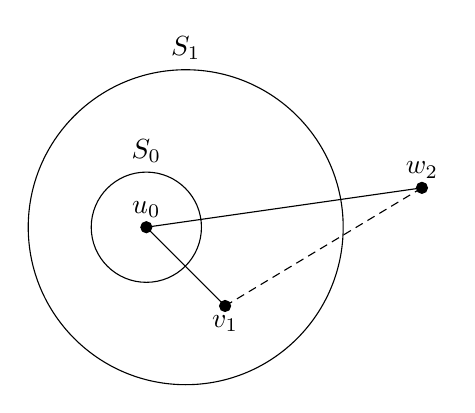
\begin{tikzpicture}
        \draw (0, 0)    circle (2)   (0, 2) node [above] {$S_1$};
        \draw (-0.5, 0) circle (0.7) (-0.5, 0.7) node [above] {$S_0$};
        \draw (-0.5, 0) circle (0.07) [fill] node [above] {$u_0$};
        \draw (0.5, -1) circle (0.07) [fill] node [below] {$v_1$};
        \draw (3, 0.5)  circle (0.07) [fill] node [above] {$w_2$};
        \draw (-0.5, 0) -- (0.5, -1)
              (-0.5, 0) -- (3, 0.5);
        \draw[densely dashed]      (0.5, -1) -- (3, 0.5);
    \end{tikzpicture}
    \caption{Proof visualization of lemma \ref{l:gnp-connectivity}}
    \label{fig:gnp-l1}
\end{figure}

\todo{
    \begin{proof}[Proof (Idea)] This is proven by induction on the subsets of a given graph G, and is visualized in figure [\ref{fig:gnp-l1}]:
        \begin{itemize}
            \item Base step: In $S_0$ there is only the node $u_0$, by hypothesis there must be an edge from $u_0$ to an arbitrary node $v_1 \in V \setminus S$;
            \item Inductive step: Go on expanding the frontier (the set of nodes in $S$ that have an edge connecting them to a node in $V \setminus S$) until the BFS visit reaches all the nodes. \qedhere
        \end{itemize}
    \end{proof}

    Note: Actually prove it by contrapositive, should be much easier
}

With this lemma, a claim on connectivity can be made:

\begin{theorem}[Connectivity of $G(n,p)$]\label{thm:gnp-connectivity}
    Let $G$ be a graph generated by $\ergen(n, p)$. If $p \geq \frac{8 \ln n}{n}$, then $G$ is connected with probability at least $1 - \frac{1}{n}$. %$\Pr[G \text{ is connected}] = 1 - \oneover{n}$
\end{theorem}

\begin{proof}
    Let $\xi_S$ be the event ``there are no edges crossing the bipartition $(S, V \setminus S)$ of the graph $G$'' for each proper nonempty subset $S$ of $V$. By the previous lemma, we can deduce that that:
    \[
        \Pr[G \text{ is not connected}] = \Pr\left[\bigvee_{S \subset V} \xi_S\right]
    \]
    
    Note that there are $2^n - 2$ of such subsets, but we are interested only in half of the corresponding events, since each event $\xi_S$ will have another event $\xi_{V \setminus S}$ that is essentially the same: in other words,  $\xi_S$ and $\xi_{V \setminus S}$ are not independent. To correct this caveat it is sufficient to only consider one fixed half of the events, and here they are conveniently chosen such that $|S| \leq \frac{|V|}{2}$.
    
    Let $n = |V|$ and $s = |S|$. Observe that there are $|S| \cdot |V \setminus S|$ possible edges from $S$ to $V \setminus S$, each of which will not be in the graph with probability $1 - p$; also, since $S$ is a subset of $V$, then $|S| \cdot |V \setminus S| = s \cdot (n - s)$. Putting the pieces together, the probability of a single event $\xi_S$ is obtained as:
    \begin{align*}
        \Pr[\xi_S] &= (1 - p)^{s \cdot (n - s)}                 & \\
        &\leq e^{-p \cdot s \cdot (n - s)}                      & \text{(by inequality \ref{eq:e-x})} \\
        &\leq e^{-p \cdot s \cdot \frac{n}{2}}                  & \text{(since $s \leq \frac{n}{2}$)} \\
        &\leq e^{-\frac{8 \ln n}{n} \cdot s \cdot \frac{n}{2}}  & \\
        &= \left(e^{-\ln n} \right)^{4 s} = n^{-4 s}            & 
    \end{align*}
    
    Now, let's fix $s$ to a specific value, and consider the probability that $\xi_S$ happens for any $S \subset V$ with cardinality $s$:
    \begin{align*}
        \Pr\left[\exists S \in \binom{V}{s} : \xi_S\right] &\leq \sum_{S \in \binom{V}{s}} \Pr[\xi_S] & \text{(by the \ref{eq:union-bound})} \\
        &\leq \sum_{S \in \binom{V}{s}} n^{-4s} = \binom{n}{s} \cdot n^{-4s}            & \text{(since $\displaystyle \abs{\binom{V}{s}} = \binom{n}{s}$)} \\
        &\leq n^s \cdot n^{-4s} = n^{-3s}                                               & \text{(since $\displaystyle \binom{n}{s} \leq n^s)$}
    \end{align*}
    
    Now we are ready to compute the probability that a graph $G$ obtained using $\ergen(n, p)$ is connected. To this purpose, the previous result is exploited once all the subsets $S$ are collected in \emph{buckets} according to their cardinality:
    \begin{align*}
        \Pr[G \text{ is not connected}] &= \Pr\left[\bigvee_{S \subset V} \xi_S\right]  & \\
        &= \sum_{s = 1}^{n/2}\Pr\left[\exists S \in \binom{V}{s} : \xi_S\right]         & \text{(disjoint probabilities)} \\
        &\leq \sum_{s = 1}^{n/2} n^{-3s}                                                & \text{(by the previous result)} \\
        &\leq \sum_{s = 1}^{n/2} n^{-3} = \oneover{2n^2}                                &
    \end{align*}
    
   By complementing the result, it entails that $\Pr[G \text{ is connected}] \geq 1 - \oneover{2n^2} \geq 1 - \oneover{n}$, which is even a stronger claim than the one stated by the theorem.
\end{proof}

The above theorem is also known as a \emph{zero-one law}: it holds for the given bound of $p$, but it ceases to hold almost immediately when $p$ crosses it: this value $p = \frac{8 \ln n}{n}$ effectively acts as a reference threshold between generators $\ergen(n, p)$ that reliably produce connected graphs and generators that reliably produce disconnected graphs.

We won't prove exactly what we just claimed, since it would be hard, but something weaker:
\begin{theorem}
    If $p < \frac{\varepsilon}{n} \ll \frac{8 \ln n}{n}$, then $G(n, p)$ is disconnected with probability $\geq 1 - \varepsilon$.
\end{theorem}

\begin{proof}
    Let $X := \deg(i)$ and $X_j$ defined as before (see [\ref{sec:gnp-degree}]).
    \begin{itemize}
        \item $X = \sum_{j \neq i} x_j = \sum_{j \neq i} \Pr{\{i, j\} \in E(G)}$;
        \item We know by hypothesis that $\expect(x_j) = p < \frac{\varepsilon}{n}$;
        \item $\expect(X) = (n - 1)p < (n - 1) \frac{\varepsilon}{n}$, just as before;
        \item $\Pr[X \geq \oneover{\varepsilon} \cdot \expect(X)] \leq \varepsilon$, by Markov's inequality \ref{eq:markov2};
        \item Since $\oneover{\varepsilon} \cdot \expect(X) \approx 1$ and $X$ has integer values, we can write the previous expression as $\Pr{X > 0} \leq \varepsilon$, and this is the probability that there is a node $i$ having at least one neighbour;
        \item Thus, by complement, $\Pr{\exists\ i : i \in V \text{ and } i \text{ has 0 neighbors}} = \Pr{G(n,p) \text{ is not connected}} \geq 1 - \varepsilon$.
    \end{itemize}
\end{proof}
    

\subsection{Diameter}

It is known that graphs generated by $\ergen(n,p)$ have small diameter with high probability. The proof is left as an exercise.


\section[Preferential attachment]{Preferential attachment\raisebox{.3\baselineskip}{\normalsize\footnotemark}}
\footnotetext{Part of this section is taken from \href{https://github.com/Halolegend94/uni_social_behavioral_networks/blob/master/chapters/ch04-random-graphs.tex}{this repo} by \href{https://github.com/Halolegend94}{Cristian Di Pietrantonio}.}\label{sec:pref-att}

\begin{figure}[ht]
    \centering
    \begin{tikzpicture}[node distance = 30mm]
        \tikzstyle{vtx}=[draw, circle, minimum size = 3em]
        
        \draw[->]
            node (a) [vtx] {$1$}
            node (b) [vtx, right of = a] {$2$}
            node (c) [vtx, right of = b] {$3$}
            node (d) [vtx, right of = c] {$N-1$}
            node (e) [vtx, right of = d] {$N$}
            node (k) [right of = c, node distance = 15mm]{$\dots$}
              
            (a) edge [loop left] ()
            (a) edge (b)
            (a) edge [bend right] (c)
            (c) edge [bend left] (d)
            (a) edge [bend left] (e)
        ;
        
    \end{tikzpicture}
    \caption{A graph generated by the standard preferential attachment model}
    \label{fig:pref-att}
\end{figure}

\emph{Preferential attachment} is another sequential model for generating random graphs, which specifically exemplifies the rule ``rich people get richer'': by adding new nodes to network, other existing nodes with higher degree will see it increase more consistently. The rule used to build a graph is the following: begin with a single vertex with a loop, then for each newly added vertex $v$, connect it to a node $i$ chosen with probability proportional to $i$'s degree. An example of such a graph is depicted in figure \ref{fig:pref-att}. Many variants of this model have been devised, such as creating $k$ edges instead of one on each step, or forbidding loops.

The graphs generated by the preferential attachment model follow a \emph{power law} degree distribution, which is also observed in many real world networks: 

\begin{definition}[Power law]
    A power law is a functional relationship $y = ax^{-c}$ between two quantities, where one quantity varies as a power of the other.
\end{definition}

Indeed, the fraction of nodes of degree $x$ approaches $x^{-3}$. This is what makes it desirable in modeling social and biological networks, and makes efficient algorithm design on such networks possible and practical. As a consequence, a power law appears as a line on a logarithmic-scaled plot, as can be seen in figure \ref{fig:power-law}.

\begin{figure}[ht]
    \centering
    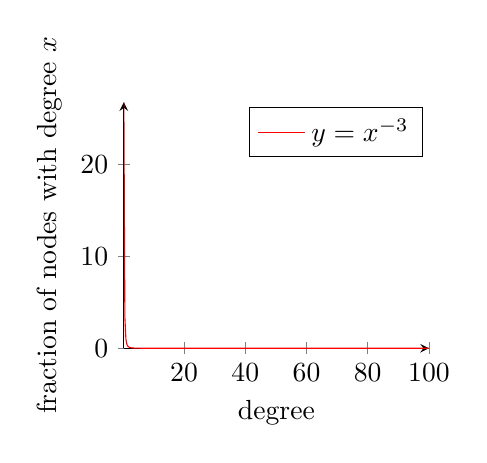
\begin{tikzpicture}
        \begin{axis}[
            width=0.45\textwidth,
            axis lines = left,
            xlabel = degree,
            ylabel = {fraction of nodes with degree $x$},
        ]
        \addplot [
            domain=0:100, 
            samples=300, 
            color=red,
        ]{1/(x^3)};
        \addlegendentry{$y=x^{-3}$}
        \end{axis}
    \end{tikzpicture}
    \hskip 0.05\textwidth
    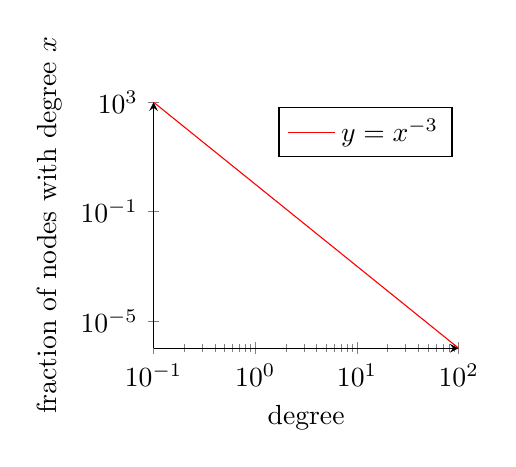
\begin{tikzpicture}
        \begin{axis}[
            width=0.45\textwidth,
            xmode=log,
            ymode=log,
            axis lines = left,
            xlabel = degree,
            ylabel = {fraction of nodes with degree $x$},
        ]
        \addplot [
            domain=0.1:100,
            samples=300,
            color=red,
        ]{1/(x^3)};
        \addlegendentry{$y=x^{-3}$}
        \end{axis}
    \end{tikzpicture}
    \caption{Power law distribution on linear and logarithmic scales}
    \label{fig:power-law}
\end{figure}

In the social network context it means that it is exponentially more likely to pick ``normal people'' with few friends or followers rather than popular profiles, called \emph{celebrities} or \emph{authorities}. Nodes with high degree in a social network are few, but they exist. So, as an example, an advertisement agency could pay those celebrities to publicize a product, enabling a spread of information due to the high number of connections those nodes have.

The actual algorithm $\pagen(n)$ constructing a graph using preferential attachment is of the inductive type:

\begin{lstlisting}[caption = {The $\pagen(n)$ algorithm}, label = {lst:algopa}]
algorithm $\pagen(n)$:
    $V \gets \{1\}$
    $E \gets \{\{1, 1\}\}$
    $\forall i \in [n] \setminus \{1\}$
        $V \gets V \cup \{i\}$
        $J \sim \randdist(V) : \Pr[J = j] = \frac{\deg(j)}{2|E| + 1}$ // NOTE: $\Pr[J = i]$ is forced to be $\oneover{2|E| + 1}$
        $j \pickUAR J$
        $E \gets E \cup \{\{i, j\}\}$
    return $G := (V, E)$
\end{lstlisting}


Note that there are many possible configurations from the second step onwards, and the probability of each of them depends on the degrees of the nodes (where a loop counts twice and a self loop once). The possible configurations with their respective probabilities are shown in figure [\ref{fig:pref-att-steps}].

\begin{figure}[ht]
    \centering
    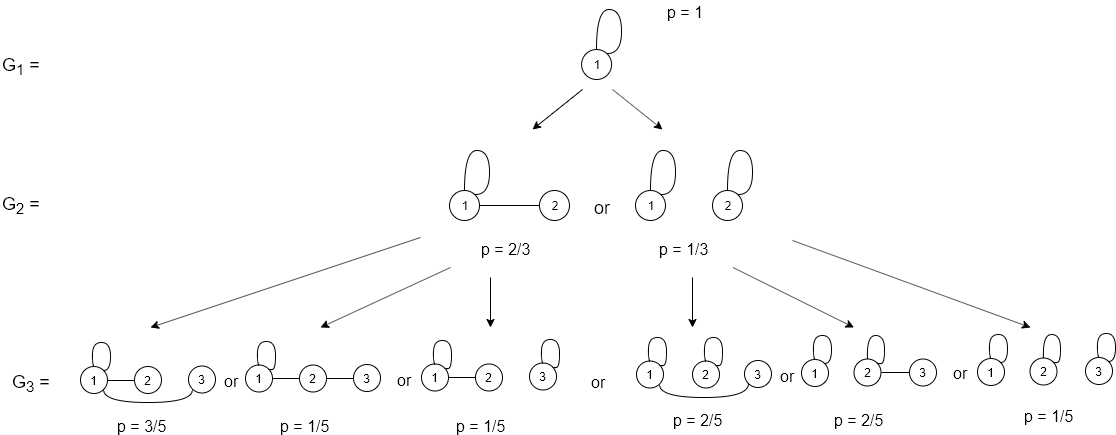
\includegraphics[width=\textwidth]{pref-attach-steps}
    \caption{Example of a graph generated by the preferential attachment model}
    \label{fig:pref-att-steps}
\end{figure}


\subsection{Degree distribution}\label{sec:pref-attach-degree}

As with the Erd\H{o}s-Rényi model, analysis starts from the distribution of its vertices' degrees; it'll turn out that such distribution indeed follows a power law. Let $G_t$ be a graph generated by the model with $t$ vertices, gathering some basic facts:
       
\begin{itemize}
    \item $\abs{V(G_t)} = \abs{E(G_t)} = t$;
    \item $\forall v \in V \quad \deg(V) > 0$
    \item Given a graph $G_t$ and a random vertex V: $\Pr[v_t \sim V] = \frac{\deg_{G_{t - 1}}(V)}{2t + 1}$, with the added rule that $\Pr[v_t \sim v_t] = \oneover{2t + 1}$.
\end{itemize}
    
\begin{theorem}\label{thm:pref-attach-degree}
    Let $X_t^{(d)}$ be the number of nodes that have degree $d$ in $G_t$. Then:
    \[
        \expect(X_t^{(d)}) = \frac{4 t}{(d + 2)(d + 1)d} \pm O(1)
    \]
\end{theorem}

\begin{observation}
    Note that, as the degree grows arbitrarily large, the number of vertices having such degree drop cubically.
\end{observation}
    
\begin{proof}
    The proof will be structured as a nested double induction: the outer one goes over the degree $d$, whereas the inner deals with the number of vertices $t$. It is worth to begin with a high level overview of what happens whenever a new vertex $v_t$ is added, and how the degree counts change after addition:

    \begin{itemize}
        \item Counting nodes with degree 1:
            \begin{itemize}
                \item $v_t$ creates a self loop: the number of nodes with degree 1 does not change;
                \item $v_t$ connects to a node $w$ of degree 1: in this case $v_t$ is a new node with degree 1, but $w$ now has a degree greater than 1, thus the overall number of nodes with degree 1 does not change;
                \item $v_t$ connects to a node of degree 2 or more: $v_t$ is a new node with degree 1, so the number of nodes with degree 1 increases by one;
            \end{itemize}
        \item Counting nodes with degree 2:
            \begin{itemize}
                \item $v_t$ creates a self loop: the number of nodes with degree 2 increases by one;
                \item $v_t$ connects to a node $w$ of degree 1: the number of nodes with degree 2 increases by one because of $w$;
                \item $v_t$ connects to a node $w$ of degree 2: the number of nodes with degree 2 decreases by 1, again because of $w$;
                \item $v_t$ connects to a node of degree 3 or more: the number of nodes with degree 2 does not change;
            \end{itemize}
        \item Counting nodes with degree $d = 3$ or greater:
            \begin{itemize}
                \item $v_t$ connects to a node $w$ of degree $d - 1$: the number of nodes with degree $d$ increases by one because of $w$;
                \item $v_t$ connects to a node $w$ of degree $d$: the number of nodes with degree $d$ decreases by one, again because of $w$;
                \item $v_t$ connects to any other node: the number of nodes with degree $d$ does not change.
            \end{itemize}
    \end{itemize}

    This list of observation will prove most useful during the rest of the proof, and will be used in designing conditioned outcome spaces, yielding in turn concrete expressions in $d$ and $t$

    \vbox{}
    
    \fbox{\textsc{Degree 1}}

    \vbox{}
        
    Since $G_{t + 1}$ depends on $G_t$, $\forall\ t = 1,2,\ldots$, we will need to condition on all the previous random choices.

    \begin{lemma}\label{l:pref-att-1}
        $\displaystyle \expect(X_{t + 1}^{(1)} \knowing X_t^{(1)} = x) = (x + 1) \left( 1 - \oneover{2t + 1} \right)$
    \end{lemma}

    \begin{proof}
        \begin{align*}
             &\ \expect(X_{t + 1}^{(1)} \knowing X_t^{(1)} = x)                                 & \phantom{mmmmmmmmmm} \\
            =&\ x \Pr[X_{t + 1}^{(1)} = x \knowing X_t^{(1)} = x] + (x + 1) \Pr[X_{t + 1}^{(1)} = x + 1 \knowing X_t^{(1)} = x] & \\
            =&\ x \frac{x + 1}{2t + 1} + (x + 1) \left( 1 - \frac{x + 1}{2t + 1} \right)        & \mathllap{\text{(Number of 1-degree vertices is known by condition)}} \\
            =&\ (x + 1) \left( \frac{x}{2t + 1} + 1 - \frac{x + 1}{2t + 1} \right)              & \\
            =&\ (x + 1) \left( 1 + \frac{x - x - 1}{2t + 1} \right)                             & \\
            =&\ (x + 1) \left( 1 - \oneover{2t + 1} \right)                                     &
        \end{align*}
    \end{proof}

    \begin{lemma}\label{l:pref-att-2}
        $\displaystyle \expect(X_{t + 1}^{(1)}) = (\expect(X_t^{(1)}) + 1)  \left(1 - \oneover{2t + 1} \right)$
    \end{lemma}

    \begin{proof}
        \begin{align*}
             &\ \expect(X_{t + 1}^{(1)})                                                            & \\
            =&\ \sum_{x \geq 0} \Pr[X_t^{(1)} = x] \expect(X_{t + 1}^{(1)} \knowing X_t^{(1)} = x)  & \text{(by total expectation)} \\
            =&\ \sum_{x \geq 0} \Pr[X_t^{(1)} = x] (x + 1) \left( 1 - \oneover{2t + 1} \right)      & \text{(by lemma [\ref{l:pref-att-1}])} \\
            =&\ \left( 1 - \oneover{2t + 1} \right) \sum_{x \geq 0} (x + 1) \Pr[X_t^{(1)} = x]      & \\
            =&\ \left( 1 - \oneover{2t + 1} \right) \left( \sum_{x \geq 0} x \Pr[X_t^{(1)} = x] + \sum_{x \geq 0} \Pr[X_t^{(1)} = x] \right)    & \text{(by distributive law)} \\
            =&\ \left( 1 - \oneover{2t + 1} \right) (\expect(X_t^{(1)}) + 1)                        & \mathllap{\text{(Def. of expected value, and law of total prob.)}}
        \end{align*}
    \end{proof}

    \begin{lemma}[Induction with degree 1]\label{l:pref-att-3} Substituting $d = 1$ in the original statement:
        \[
            \expect(X_t^{(1)}) = \frac{4 t}{3 \cdot 2 \cdot 1} \pm O(1) = \frac{2}{3} t \pm O(1)
        \]
        or in a different formulation:
        \[
            \exists\ c > 0\; \forall\ t\geq 0 \quad \frac{2}{3} (t + 1) - c \leq \expect( X_{t + 1}^{(1)} ) \leq \frac{2}{3} (t + 1) + c
        \]
    \end{lemma}

    \begin{proof}

        \begin{itemize}
            \item Base: ($t = 0$): At time $t + 1 = 1$ the graph is composed by a single node with degree 2, thus no 1-degree vertex is present. The claim holds for $c \geq \frac{2}{3}$:
            \[
                \frac{2}{3} - c \leq \expect(X_1^{(1)}) = 0 \leq \frac{2}{3} + c
            \]

            \item Induction -- upper bound:
            \begin{align*}
                \expect(X_{t + 1}^{(1)}) =&\ \left( \expect(X_t^{(1)}) + 1 \right) \left( 1 - \frac{1}{2t + 1} \right)  & \text{(by lemma [\ref{l:pref-att-2}])} \\
                \leq&\ \left( \frac{2}{3}t + c + 1 \right) \left( 1 - \frac{1}{2t + 1} \right)                          & \text{(by induction hypothesis)} \\
                   =&\ \frac{2}{3}t + c + 1 - \frac{2t}{6t + 3} - \frac{c + 1}{2t + 1}                                  & \\
                   =&\ \frac{2}{3} (t + 1) + c + \frac{1}{3} - \frac{2t}{6t + 3} - \frac{c + 1}{2t + 1}                 & \\
                   =&\ \frac{2}{3} (t + 1) + c + \frac{2t + 1 - 2t - 3c - 3}{6t + 3}                                    & \\
                   =&\ \frac{2}{3} (t + 1) + c + \frac{- 3c - 2}{6t + 3}                                                & \\
                \leq&\ \frac{2}{3} (t + 1) + c                                                                          & (c > 0)
            \end{align*}

            \item Induction -- lower bound:
            \begin{align*}
                \expect(X_{t + 1}^{(1)}) =&\ \left( \expect(X_t^{(1)}) + 1 \right) \left( 1 - \frac{1}{2t + 1} \right)  & \text{(by lemma [\ref{l:pref-att-2}])} \\
                \geq&\ \left( \frac{2}{3}t - c + 1 \right) \left( 1 - \frac{1}{2t + 1} \right)                          & \text{(by induction hypothesis)} \\
                   =&\ \frac{2}{3}t - c + 1 - \frac{2t}{6t + 3} + \frac{c - 1}{2t + 1}                                  & \\
                   =&\ \frac{2}{3}(t + 1) - c + \frac{1}{3} - \frac{2t}{6t + 3} + \frac{c - 1}{2t + 1}                  & \\
                   =&\ \frac{2}{3}(t + 1) - c + \frac{2t + 1 - 2t + 3c - 3}{6t + 3}                                     & \\
                   =&\ \frac{2}{3}(t + 1) - c + \frac{3c - 2}{6t + 3}                                                   & \\
                \geq&\ \frac{2}{3}(t + 1) - c                                                                           & \text{(for $c \geq \frac{2}{3}$)}
            \end{align*}

        \end{itemize}
    \end{proof}

    \vbox{}
    
    \fbox{\textsc{Degree 2}}

    \vbox{}

    \begin{lemma}\label{l:pref-att-4}
        $\displaystyle \expect(X_{t + 1}^{(2)} \knowing X_t^{(2)} = x \wedge X_t^{(1)} = y) = x \left( 1 - \frac{2}{2t + 1} \right) + \frac{y + 1}{2t + 1}$
    \end{lemma}

    \begin{proof}
        \begin{align*}
            &\ \expect(X_{t + 1}^{(2)} \knowing X_t^{(2)} = x \wedge X_t^{(1)} = y)                                                         & \\
            =&\ (x - 1) \Pr[X_{t + 1}^{(2)} = x - 1 \knowing X_t^{(2)} = x \wedge X_t^{(1)} = y]                                            & \\
            &\; + x \Pr[X_{t + 1}^{(2)} = x \knowing X_t^{(2))} = x \wedge X_t^{(1)} = y]                                                   & \\
            &\; + (x + 1) \Pr[X_{t + 1}^{(2)} = x + 1 \knowing X_t^{(2)} = x \wedge X_t^{(1)} = y]                                          & \\
            =&\ (x - 1) \left( x \frac{2}{2t + 1} \right)                                                                                   & \\
            &\; + x \left( 1 - x \frac{2}{2t + 1} - y \frac{1}{2t + 1} - \frac{1}{2t + 1} \right)                                           & \\
            &\; + (x + 1) \left( y \frac{1}{2t + 1} + \frac{1}{2t + 1} \right)                                                              & \\
            =&\ (x - 1) \frac{2x}{2t + 1} + x \left( 1 - \frac{2x - y - 1}{2t + 1} \right) + (x + 1) \left( \frac{y + 1}{2t + 1} \right)    & \\
            =&\ \frac{(x - 1) {2x} + x \left( 2t + 1 - 2x - y - 1 \right) + (x + 1) \left( {y + 1} \right)}{2t + 1}                         & \\
            =&\ \frac{2x^2 - 2x + 2tx - 2x^2 - xy + xy + x + y + 1}{2t + 1}                                                                 & \\
            =&\ \frac{1 - x + 2tx + y}{2t + 1}                                                                                              &
        \end{align*}
    \end{proof}

    \begin{lemma}\label{l:pref-att-5}
        $\displaystyle \expect(X_{t + 1}^{(2)}) = \expect(X_t^{(2)}) \left( 1 - \frac{2}{2t + 1} \right) + \frac{\expect(X_t^{(1)}) + 1}{2t + 1}$
    \end{lemma}
    \todo{
        No idea on this...

        \begin{proof}
            It is possible to prove this lemma explicitly with a procedure similar to the one used for lemma [\ref{l:pref-att-2}], but here we will present a more compact (implicit) proof:
            \[
                E_{X_t^{(2)}=x} \left[ E_{X_t^{(1)}=y : X_t^{(2)}=x} \left[ x \cdot \left( 1 - \frac{2}{2t+1} \right) + \frac{y+1}{2t+1} \right] \right]
            \]
            Note that this is possible because the expected value is linear and (in this case) also its value is linear with respect to $x$ and $y$.
        \end{proof}
    }
    

    Now we are going to use the bounds found for $\expect(X_t^{(1)})$ in lemma [\ref{l:pref-att-3}] to prove similar bounds for $\expect(X_t^{(2)})$.
    
    \begin{lemma}[Induction with degree 2]\label{l:pref-att-6} Substituting $d = 2$ in the original statement:
        \[
            \expect(X_t^{(2)}) = \frac{4 t}{4 \cdot 3 \cdot 2} \pm O(1) = \frac{1}{6} t \pm O(1)
        \]
        or in a different formulation:
        \[
            \exists\ c > 0\; \forall\ t\geq 0 \quad \frac{1}{6} (t + 1) - c \leq \expect( X_{t + 1}^{(2)} ) \leq \frac{1}{6} (t + 1) + c
        \]
    \end{lemma}

    \begin{proof}

        \begin{itemize}
            \item Base: ($t = 0$): At time $t + 1 = 1$ the graph is composed by a single node with degree 2, thus exactly one 2-degree vertex is present. The claim holds for $c \geq \frac{5}{6}$:

            \[
                \frac{1}{6} - c \leq \expect(X_1^{(2)}) = 1 \leq \frac{1}{6} + c
            \]

            \item Induction -- upper bound:
                \begin{align*}
                    \expect(X_{t + 1}^{(2)}) =&\ \expect(X_t^{(2)}) \cdot \left( 1 - \frac{2}{2t + 1} \right) + \frac{\expect(X_t^{(1)}) + 1}{2t + 1} & \text{(by lemma [\ref{l:pref-att-5}])} \\
                    \leq&\ \left( \frac{1}{6} t + c \right) \cdot \left( 1 - \frac{2}{2t + 1} \right) + \frac{\frac{2}{3}t + c + 1}{2t + 1} &
                    \text{(\parbox{\textwidth/3}{by inductive hypothesis and upper bound of [\ref{l:pref-att-3}]})} \\
                       =&\ \frac{1}{6} t + c + \frac{-\frac{1}{3} t - 2c + \frac{2}{3} t + c + 1}{2t + 1}                                   & \\
                       =&\ \frac{1}{6} t + c + \frac{ \frac{1}{3} t - c + 1}{2t + 1}                                                        & \\
                       =&\ \frac{1}{6} t + c + \frac{ \frac{1}{3} t + \frac{1}{6}}{2t + 1} + \frac{ - c + \frac{5}{6}}{2t + 1}              & \\
                       =&\ \frac{1}{6} t + c + \frac{1}{6} + \frac{ \frac{5}{6} - c}{2t + 1}                                                & \\
                       =&\ \frac{1}{6} (t + 1) + c + \frac{ \frac{5}{6} - c}{2t + 1}                                                        & \\
                    \leq&\ \frac{1}{6} (t + 1) + c                                                                                          & \text{(for $c \geq \frac{5}{6}$)}
                \end{align*}

            \item Induction -- lower bound:
                \begin{align*}
                    \expect(X_{t + 1}^{(2)}) =&\ \expect(X_t^{(2)}) \cdot \left( 1 - \frac{2}{2t + 1} \right) + \frac{\expect(X_t^{(1)}) + 1}{2t + 1} & \text{(by lemma [\ref{l:pref-att-5}])} \\
                    \geq&\ \left( \frac{1}{6} t - c \right) \cdot \left( 1 - \frac{2}{2t + 1} \right) + \frac{\frac{2}{3}t - c + 1}{2t + 1} &
                    \text{(\parbox{\textwidth/3}{by inductive hypothesis and lower bound of [\ref{l:pref-att-3}]})} \\
                       =&\ \frac{1}{6} t - c + \frac{-\frac{1}{3} t + 2c + \frac{2}{3} t - c + 1}{2t + 1}                                   & \\
                       =&\ \frac{1}{6} t - c + \frac{ \frac{1}{3} t + c + 1}{2t + 1}                                                        & \\
                       =&\ \frac{1}{6} t - c + \frac{ \frac{1}{3} t + \frac{1}{6}}{2t + 1} + \frac{c + \frac{5}{6}}{2t + 1}                 & \\
                       =&\ \frac{1}{6} t - c + \frac{1}{6} + \frac{ \frac{5}{6} + c}{2t + 1}                                                & \\
                       =&\ \frac{1}{6} (t + 1) - c + \frac{ \frac{5}{6} + c}{2t + 1}                                                        & \\
                    \geq&\ \frac{1}{6} (t + 1) - c                                                                                          & (c > 0)
                \end{align*}

        \end{itemize}
    \end{proof}

    \vbox{}
    
    \fbox{\textsc{Degree 3+}}

    \vbox{}

    \begin{lemma}\label{l:pref-att-7}\footnote{Notice how the third term in [\ref{l:pref-att-4}] is absent here: self loops do not affect the number of nodes of degree greater than 2}
        $\displaystyle \expect(X_{t + 1}^{(d)} \knowing X_t^{(d)} = x \wedge X_t^{(d - 1)} = y) = x \left( 1 - \frac{d}{2t + 1} \right) + y \frac{d - 1}{2t + 1}$
    \end{lemma}

    \begin{proof}
        \begin{align*}
            &\ \expect(X_{t + 1}^{(d)} \knowing X_t^{(d)} = x \wedge X_t^{(d - 1)} = y)             & \\
            =&\  (x + 1) \Pr[X_{t + 1}^{(d)} = x + 1 \knowing X_t^{(2)} = x \wedge X_t^{(1)} = y]   & \text{(a new $d$-degree vertex is added)} \\
             &\; + (x - 1) \Pr[X_{t + 1}^{(d)} = x - 1 \knowing X_t^{(2)} = x \wedge X_t^{(1)} = y] & \text{(a $d$-degree vertex is lost)} \\
             &\; + x \Pr[X_{t + 1}^{(d)} = x \knowing X_t^{(2)} = x \wedge X_t^{(1)} = y]           & \mathllap{\text{(the number of $d$-degree vertices is unchanged)}} \\
            =&\ (x + 1) \frac{d - 1}{2t + 1} y                                                      & \\
             &\; + (x - 1) \frac{d}{2t + 1} x                                                       & \\
             &\; + x \left( 1 - \frac{d - 1}{2t + 1} y - \frac{d}{2t + 1} x \right)                 & \\
            =&\ \frac{(x + 1)(d - 1)y + (x - 1)dx + x(2t + 1) - x(d - 1)y - dx^2}{2t + 1}           & \\
            =&\ \frac{y(d - 1)(x + 1 - x) + x(d(x - 1) + 2t + 1 - dx)}{2t + 1}                      & \\
            =&\ \frac{y(d - 1) + x(dx  - d + 2t + 1 - dx)}{2t + 1}                                  & \\
            =&\ \frac{y(d - 1) + x(1 - d + 2t)}{2t + 1}                                             & \qedhere
        \end{align*}
    \end{proof}

    \begin{lemma}\label{l:pref-att-8}
        $\displaystyle \expect(X_{t + 1}^{(d)}) = \expect(X_t^{(d)}) \cdot \left( 1 - \frac{d}{2t + 1} \right) + \expect(X_t^{(d - 1)}) \cdot \frac{d - 1}{2t + 1}$
    \end{lemma}

    \begin{proof}
        It is possible to prove this lemma explicitly as we did for lemma [\ref{l:pref-att-2}], or implicitly as we did for lemma [\ref{l:pref-att-5}].
    \end{proof}

    \begin{lemma}[Induction with degree 3+]\label{l:pref-att-9} Assuming $d \geq 3$:
        \[
            \expect(X_t^{(d)}) = \frac{4 t}{(d + 2)(d + 1)d} \pm O(1)
        \]
        or in a different formulation:
        \[
            \exists\ c > 0\; \forall\ t \geq 0 \quad \frac{4(t + 1)}{(d + 2)(d + 1)d} - c \leq \expect(X_{t + 1}^{(1)}) \leq \frac{4(t + 1)}{(d + 2)(d + 1)d} + c
        \]
    \end{lemma}

    \begin{proof}
        
        \todo{To be verified, adjusting the bound on $c$
        
            Base: ($t = 0$): At time $t + 1 = 1$ the graph is composed by a single node with degree 2, thus no vertex wih degree 3 or greater is present. The claim holds for $c \geq 1$:

            \[
                \frac{4}{(d + 2)(d + 1)d} - c \leq \expect(X_1^{(d)}) = 0 \leq \frac{4}{(d + 2)(d + 1)d} + c
            \]

        }

        \begin{itemize}

            \item Induction -- upper bound:

            % Small hack required to place a todo 
            \leavevmode \todo{Ugly...

                \scriptsize\begin{align*}
                    \expect(X_{t + 1}^{(d)}) =&\ \expect(X_t^{(d)}) \left( 1 - \frac{d}{2t + 1} \right) + \expect(X_t^{(d - 1)}) \frac{d - 1}{2t + 1} & \text{(by lemma [\ref{l:pref-att-8}])} \\
                    \leq&\ \left( \frac{4t}{(d + 2)(d + 1)d} + c \right) \left( 1 - \frac{d}{2t + 1} \right) + \left( \frac{4t}{(d + 1)(d - 1)d} + c \right)  \frac{d - 1}{2t + 1} & \text{(by induction hypothesis)} \\
                       =&\ \frac{4t}{(d + 2)(d + 1)d} \left( 1 - \frac{d}{2t + 1} \right) + \frac{4t}{(d + 1)(d - 1)d} \cdot \frac{d - 1}{2t + 1} + c \left( 1 - \frac{d}{2t + 1} + \frac{d - 1}{2t + 1}\right) & \\
                       =&\ \frac{4t}{(d + 2)(d + 1)d} \left( 1 - \frac{d}{2t + 1} \right) + \frac{4t}{(d + 1)d(2t + 1)} + c \left( 1 - \frac{1}{2t + 1}\right) & \\
                    \leq&\ \frac{4t}{(d + 2)(d + 1)d} \left( 1 - \frac{d}{2t + 1} \right) + \frac{4t}{(d + 1)d(2t + 1)} + c & (1 - \frac{1}{2t + 1} < 1) \\
                       =&\ \frac{4t}{(d + 2)(d + 1)d} - \frac{4t}{(d + 2)(d + 1)(2t + 1)} + \frac{4t}{(d + 1)d(2t + 1)} + c & \\
                       =&\ \frac{4t}{(d + 2)(d + 1)d} + \frac{4t}{(d + 1)(2t + 1)} \cdot \frac{- d + d + 2}{(d + 2)d} + c & \\
                       =&\ \frac{4t}{(d + 2)(d + 1)d} + \frac{8t}{(2t + 1)(d + 2)(d + 1)d} + c & \\
                    \leq&\ \frac{4t}{(d + 2)(d + 1)d} + \frac{8t + 4}{(2t + 1)(d + 2)(d + 1)d} + c & \text{(\parbox{\textwidth/3}{adding 4 allows simplification without compromising the upper bound})} \\
                       =&\ \frac{4t}{(d + 2)(d + 1)d} + \frac{4}{(d + 2)(d + 1)d} + c & \\
                       =&\ \frac{4(t + 1)}{(d + 2)(d + 1)d} + c &
                \end{align*}
            }

            \item Induction -- lower bound:

            \leavevmode \todo{...stuff

                \scriptsize\begin{align*}
                    \expect(X_{t + 1}^{(d)}) =&\ \expect(X_t^{(d)}) \left( 1 - \frac{d}{2t + 1} \right) + \expect(X_t^{(d - 1}) \frac{d - 1}{2t + 1} & \text{(by lemma [\ref{l:pref-att-8}]} \\
                    \geq&\ \left( \frac{4t}{(d + 2)(d + 1)d} - c \right) \left( 1 - \frac{d}{2t + 1} \right) + \left( \frac{4t}{(d + 1)(d - 1)d} - c \right) \frac{d - 1}{2t +1 } & \text{(by induction hypothesis)} \\
                       =&\ \frac{4t}{(d + 2)(d + 1)d} \left( 1 - \frac{d}{2t + 1} \right) + \frac{4t}{(d + 1)(d - 1)d} \cdot \frac{d - 1}{2t + 1} - c \left( 1 - \frac{d}{2t + 1} + \frac{d - 1}{2t + 1}\right) & \\
                       =&\ \frac{4t}{(d + 2)(d + 1)d} \left( 1 - \frac{d}{2t + 1} \right) + \frac{4t}{(d + 1)d(2t + 1)} - c \left( 1 - \frac{1}{2t + 1}\right) & \\
                       =&\ \frac{4t}{(d + 2)(d + 1)d} - \frac{4t}{(d + 2)(d + 1)(2t + 1)} + \frac{4t}{(d + 1)d(2t + 1)} - c \left( 1 - \frac{1}{2t + 1}\right) & \\
                       =&\ \frac{4t}{(d + 2)(d + 1)d} - \frac{4t}{(d + 1)(2t + 1)} \left( \frac{1}{d + 2} - \frac{1}{d} \right) - c \left( 1 - \frac{1}{2t + 1}\right) & \\
                       =&\ \frac{4t}{(d + 2)(d + 1)d} - \frac{8t}{(d + 2)(d + 1)d(2t + 1)} - c \left( 1 - \frac{1}{2t + 1}\right) & \\
                       =&\ \frac{4t}{(d + 2)(d + 1)d} - \frac{8t + 4 - 4}{(d + 2)(d + 1)d(2t + 1)} - c \left( 1 - \frac{1}{2t + 1}\right) & \\
                       =&\ \frac{4t}{(d + 2)(d + 1)d} + \frac{4}{(d + 2)(d + 1)d} - \frac{4}{(d + 2)(d + 1)d(2t + 1)} - c \left( 1 - \frac{1}{2t + 1}\right) & \\
                       =&\ \frac{4(t + 1)}{(d + 2)(d + 1)d} - \frac{4}{(d + 2)(d + 1)d(2t + 1)} - c + \frac{c}{2t + 1} & \\
                       =&\ \frac{4(t + 1)}{(d + 2)(d + 1)d} - c + \frac{1}{2t + 1} \left( c - \frac{4}{(d + 2)(d + 1)d} \right) & \\
                    \geq&\ \frac{4(t + 1)}{(d + 2)(d + 1)d} - c & (*)
                \end{align*}


                In the last step, marked with $*$, the removed term is always positive for $c \geq \frac{1}{15}$, since:
                
                \[
                    \frac{4}{(d + 2)(d + 1)d} \leq \frac{4}{5 \cdot 4 \cdot 3} = \frac{1}{15} \qquad \forall d \geq 3
                \]

            }


        \end{itemize}
        
    \end{proof}

    The three lemmata \ref{l:pref-att-3}, \ref{l:pref-att-6} and \ref{l:pref-att-9} collectively satisfy the required bounds for any degree $d$, thus proving the original theorem.

\end{proof}
